\chapter{Short Introduction to Clustering}\label{ch:IntroClustering}

Firstly, we need to provide an introduction, albeit a relatively brief one, to clustering and its applications in order to ease the understanding of the following chapters. For this purpose, the study carried out in \cite{Everitt:2009:CA:1538772} serves as a basis. In Section \ref{sec:ReasonsClassif} we present the reasons that lead humans to develop automatic classification methods. The numerical formulation of the latter is shown in Section \ref{sec:NumMethClassif}. We give an intuitive definition of ``cluster'' in Section \ref{sec:WhatIsCluster}. Lastly, a list of clustering application is presented in Section \ref{sec:ClusteringApplications}.

\section{Reasons for Classifying} \label{sec:ReasonsClassif}

Classification can be understood as a way of simplifying the information contained in large datasets so that is easily understood by humans. Thus, the extraction and posterior use of the information are also simplified. If we are able to meaningfully divide a large dataset into subsets or groups, we can extract information common to elements of one of these subsets and provide a precise description that encompasses them.

The need to analyze information grows with the emergence and availability of large datasets in science. The analysis of this type of information by classification, or clustering, is known today as \textit{Data Science}. In the 21st century a particular interest in data science arose with the advent of the \textit{World Wide Web}, known as the Internet, where the aim has become to extract relevant information from the Web pages that make up this vast network.

It is important to note that, in most cases, there is no single classification criterion for the same dataset, but rather a wide variety of data. In the case of individuals, they could be classified, for example, on the basis of their income, or according to the amount of calories they consume over a defined period of time. Thus, different classification criteria do not necessarily result in the same division into groups of the set to be classified; in that way, different criteria will serve different purposes.

\section{Numerical Methods of Classification} \label{sec:NumMethClassif}

Numerical methods for clustering appeared in branches of natural sciences, such as biology or zoology, in an attempt to eliminate the subjectivity implicit in the classification of new species. The aim is to provide an objective and stable method for classifying and grouping elements.

These methods adopt different names that depend on the field in which they are applied: numerical taxonomy in biology, $Q$ analysis in psychology, or unsupervised pattern recognition in \acf{AI}. Today, however, \textit{cluster analysis} or just \textit{clustering} are the most widely accepted and extended terms for tasks that involve the discovery of subgroups within a set of elements.

In most clustering applications, the goal is to obtain a data partition, in which each instance or object belongs to a single cluster, and the union of all clusters contains all the individual objects. That said, it should be noted that, in some circumstances, solutions where there is an overlap between clusters are acceptable, or there may not be acceptable data partitions at all.

In the literature, clustering methods are often divided into two subsets: partitional clustering and hierarchical clustering. In hierarchical clustering the result is not a partition of the data with a certain number of clusters (as in partitional clustering) but instead a dendrogram in which there are partitions that include from the whole dataset to particular individuals \cite{Everitt:2009:CA:1538772}. A representative example of partitional clustering is the widely studied and well-known algorithm K-means \cite{wu2009top}, while for hierarchical clustering the \acsfont{CURE} method should be highlighted \cite{guha1998cure}. In this work we focus on partitional clustering.

The most common way to represent the data on which clustering is applied is an array $X$ of dimension $n\times u$. Each row corresponds to an instance or object to be processed, and each column corresponds to one of the variables that characterize those instances. The commonly accepted term to refer to each row is \textit{feature vector}, and the set of feature vectors is called \textit{dataset}.


$$ X = \left( \begin{array}{cccc}

x_{1,1} & x_{1,2} & \cdots & x_{1,u} \\

x_{2,1} & \cdots & \cdots & \cdots  \\

\vdots & \vdots & \vdots & \vdots \\

x_{n,1} & \cdots & \cdots & x_{n,u} \\

\end{array} \right) $$

The entry $x_{i,j}$ in $X$ corresponds to the value of the $j$th variable in the $i$th instance. We will refer to the $i$th instance in $X$ as $x_i = (x_{[i,1]}, \cdots, x_{[i,u]})$, which is a feature vector.

We can define partitional clustering as the task of grouping the instances of the dataset $X$ into $k$ clusters, so that new information can be extracted from them. A typical clustering algorithm assigns a class label $l_i$ to each instance $x_i \in X$. As a result, we obtain the set of labels $L = \{l_1, \cdots, l_n\}$, with $l_i \in \{1, \cdots, k\}$, that effectively splits $X$ into $k$ non-overlapping clusters $\{c_i, \cdots, c_k\}$ to form a partition called $C$. The criterion used to assign an instance to a given cluster is the similarity to the rest of elements in that cluster, and the dissimilarity to the rest of instances of the dataset, which can be obtained with some kind of distance measurement $d(\cdot,\cdot)$ \cite{jain1999data}.

Variables in $X$ can be a mixture of attributes in a continuous, discrete, or categorical domain. In addition, it is possible that, in real problems, some entries may not be available. This mix of variable types and missing values can complicate the clustering task. However, there are methods to deal with this, such as inference of missing values or domain transformations.

In some applications, matrix rows may contain repeated measurements of the same variable under different conditions, at different times, or even at different spatial locations. An example of this can be the height measurements of a group of children in the same month over the years. This type of data has a structure that, again, can complicate the task of clustering.

Some clustering methods involve making transformations on the $X$ matrix. They convert it into a $n \times n$ matrix that stores measurements extracted from the $X$ matrix which relate one instance to all the others (such as similarity, distance or dissimilarity).

Put simply, clustering is the discovery of groups in data, and should never be confused with methods of discrimination or assignment; these are known in \acs{AI} as Supervised Learning, as we have already mentioned in Section \ref{sec:TypesOfML}. Once the general structure of clustering methods has been defined, the next question would be: What is a cluster? Section \ref{sec:WhatIsCluster} tries to answer this question.

\section{What is a Cluster?} \label{sec:WhatIsCluster}

So far, the terms cluster, group and class have been used in a completely intuitive way, with no need for any formal definition, in a further proof of the innate nature of these concepts in the human being. In fact, giving a formal definition of cluster is a task, not only complicated, but in many occasions not very useful. For example, in \cite{lance1967general} a cluster definition that is completely dependent on user interpretation is proposed. According to this definition, a cluster is just the preconceived notion of cluster that the user already had.

\begin{quotation}{\slshape
		The value judgment of the user is the ultimate criterion for evaluating the meaning of these terms [cluster]. If using them produces an answer of value, no more need be asked of them.}
	\begin{flushright}
		\textbf{R.E. Bonner, On Some Clustering Techniques, 1964} 
	\end{flushright}
\end{quotation}

Although the definition above is accurate in a wide range of situations, a somewhat more analytical approach from the mathematical point of view is needed. A definition of cluster in terms of internal cohesion (homogeneity) and external isolation (separation) is proposed in \cite{cormack1971review} and \cite{gordon:1999}. Figure \ref{fig:ClustersProperties} informally illustrates the properties described above, so that any observer will easily spot the clusters present in it without the need for a formal definition. This may explain why achieving a mathematically accurate definition of homogeneity and separation may become unnecessary.

\begin{figure}[bth]
	\myfloatalign
	{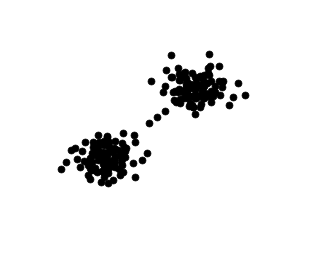
\includegraphics[width=.3\linewidth]{gfx/Clustering/TwoBasicsClusters}}
	{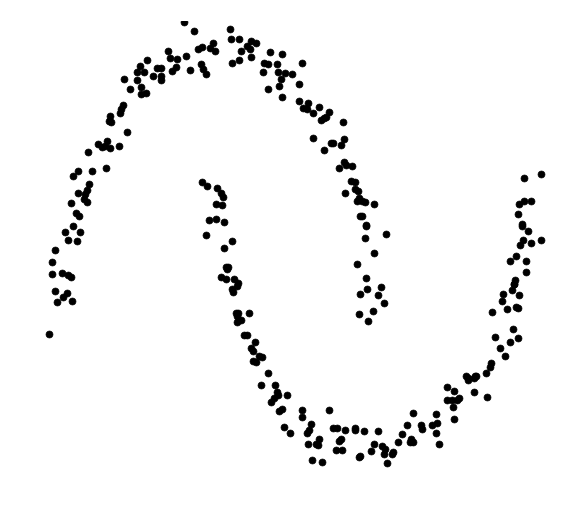
\includegraphics[width=.3\linewidth]{gfx/Clustering/MoonsBasics}}
	{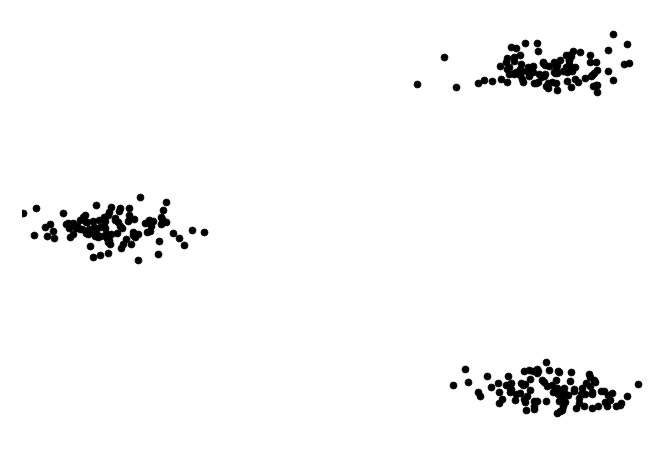
\includegraphics[width=.3\linewidth]{gfx/Clustering/ThreeBasicClusters}}
	\caption{Clusters with internal cohesion and/or external isolation.}\label{fig:ClustersProperties}
\end{figure}

It is not entirely clear how people recognize different clusters when they are represented on a plane, but one of the variables that certainly has an influence is the distribution of relative distances between objects or points.

On the other hand, as mentioned earlier in this section, it may be the case that there is no justified partition in a dataset. Figure \ref{fig:uniform_cloud} shows a dataset for which most observers would conclude that there are no distinct groups but only a cloud of uniformly distributed points. Ideally, one would expect a clustering method applied to this same dataset to reach the same conclusion.

\begin{figure}[!h]
	\centering
	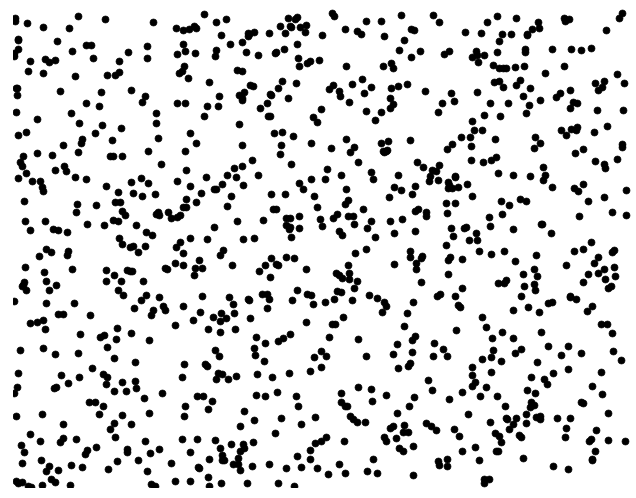
\includegraphics[scale=0.2]{gfx/Clustering/rand.png} 
	\caption{Cloud of uniformly distributed points.}\label{fig:uniform_cloud}
\end{figure}

However, most unsupervised learning methods will result in uniform partitioning as shown in Figure \ref{fig:uniform_partition}. The number of partitions will depend on the method applied, although uniform partitioning will be achieved in any case.

\begin{figure}[!h]
	\centering
	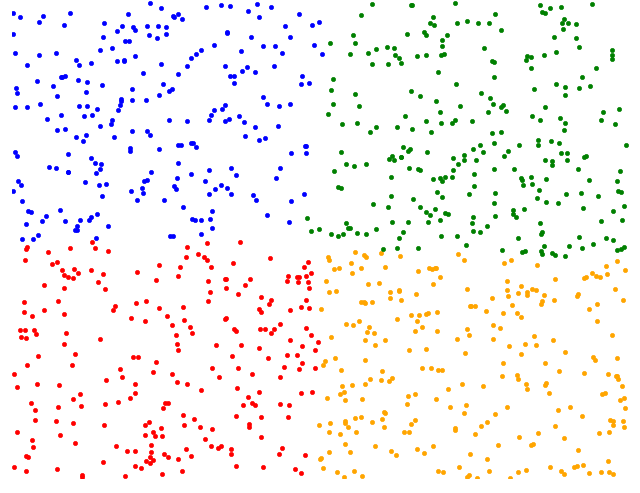
\includegraphics[scale=0.2]{gfx/Clustering/randClasif.png} 
	\caption{Classified cloud of uniformly distributed points.}\label{fig:uniform_partition}
\end{figure}

The process of dividing a homogeneous distribution of data into different groups is known as dissection, and such a process may be useful in certain circumstances. However, since in most cases the structure of the data is not known a priori, there is a risk of interpreting all solutions in terms of the existence of subgroups, which would lead to the imposition of a fictitious structure where there is none.

\section{Applications of Clustering} \label{sec:ClusteringApplications}

As has been already mentioned, the general problem clustering attempts to solve is present in many disciplines: biology, botany, medicine, psychology, geography, marketing, image processing, psychiatry, archaeology, etc. This section presents some of the applications of clustering related to these and others knowledge fields.

\subsection{Marketing}

Separating customers into homogeneous groups is one of the most common marketing tasks. A marketing manager might wonder how to group potential customers according to the potential benefits of a new product being introduced into the market. On the other hand, a marketing analyst might be interested in grouping companies according to their financial characteristics, in order to analyze them and predict their market strategies.

An example of the application of clustering in this field was published in \cite{green1967cluster}. With a large number of cities available for analysis, they had to restrict the places in which to carry out their study for economic reasons. To this end, they relied on cluster analysis to classify cities into small groups based on fourteen city features, including size and average income \textit{per capita}. Since cities in the same group were expected to be very similar, they chose one city from each of them to conduct their study.

Another application of cluster analysis in marketing was described in \cite{chakrapani2004statistics}. In this case, a car manufacturer believes that buying a sports car is not a decision based solely on economic capabilities or age, but instead a lifestyle decision made by those who decide to buy a sports car (as opposed to those who do not). Consequently, the manufacturer decides to carry out a study, using cluster analysis, to identify what types of person would buy a sports car in order to focus its marketing campaigns specifically on this sector.

\subsection{Astronomy}

Given a set of astronomical data, researchers want to know, for example, how many classes of stars are present in them according to some statistical criteria. The most frequently asked questions in this area are: How many statistically different objects are present in the data and which class should each object be assigned to? Do previously unknown classes of objects appear? Cluster analysis can be applied to answer these questions, helping to detect statistically anomalous objects, as well as to guide the process of classifying them. Examples include the discovery of high redshift quasars, type 2 quasars---highly luminous, active galactic nuclei often obscured by dust and gas---and brown dwarfs.

In \cite{faundez1996classification} a specific example of the above can be found. Clustering techniques were applied to data on the chemical composition of 192 planetary nebulae. Six different groups were identified, which were similar in many aspects to a previous classification of such objects, but also showed interesting differences that researchers had so far missed.

Clustering based on normal distributions is applied to a set of 2370 stars in \cite{celeux1992classification}. They were described by their relative speed to the galactic nucleus and galactic rotation. Using a model of three clusters, they found one cluster of large size and small volume, and two of small size and large volume.

\subsection{Psychiatry}

Mind disorders are often more difficult to diagnose than body pathologies, which is why there has been a growing interest in cluster analysis techniques to refine, or even redefine, diagnostic techniques in the field of psychiatry. Much of this work involves depressed patients, cases where the interest lies in distinguishing between two types of depression: endogenous (congenital) and neurotic.

In \cite{pledger2008using} clustering techniques are applied to 200 patients based on their answers to a questionnaire about depression, along with information about their sex, age, mental state, and illnesses. This is a clear example of different types of variables included in the same dataset. One of the groups obtained as a result of this study was identified as a marker of endogenous depression.

Cluster analysis has also been used to find a classification of individuals who attempted suicide, which could lay the groundwork for further studies on the causes and treatments of the problem. In \cite{paykel1978classification} a study on 236 cases of failed suicides recorded by the emergency service of a city in the United States of America is presented. From the set of available variables, fourteen were selected as particularly relevant for classification and, therefore, were used in the analysis. Among them were: age, number of suicide attempts, severity of depression and degree of hostility, in addition to a series of demographic features. Clustering methods were applied to the resulting dataset; the most significant result corresponds to a division into three well-defined clusters.

\subsection{Meteorology and Climatology}

Huge amounts of global weather data are collected daily. Exploring these data using clustering techniques can bring new approaches to study climatology and environmental phenomena.

In \cite{littmann2000empirical} clustering techniques are applied to data collected on daily changes in surface pressure in the Mediterranean basin, and twenty groups explaining the variance of rainfall in the central Mediterranean regions were found. Another example can be found in \cite{liu2005mining}, where the Fuzzy K-means algorithm is applied to spatial-temporal data on the climatology of southern-central regions of \acsfont{USA}. 

\subsection{Archaeology}

Archaeology is another discipline in which clustering is useful. The classification of different objects found in deposits can help to discover their use, the historical periods to which they belong, as well as the population that used them. Similarly, studying fossilized materials can help reveal how prehistorical societies lived. 

An early example of the application of clustering to archaeological objects is given in \cite{hodson1966some}, where clustering techniques are applied to a group of brooches dating from the Iron Age, producing a classification for them of proven archaeological relevance. Another example found in \cite{hodson1971numerical} is the application of the K-means algorithm to construct a taxonomy of hand axes found in the British Isles. The variables taken into account to describe each axe include length, width and pointedness. Clustering resulted in two groups of axes, one made up of small and thin axes and the other made up of large and thick axes.

Regarding fossilized materials, in \cite{sutton1995cluster} a study of 155 coprolites found at Antelope House, a prehistoric site at Chelly Canyon in Arizona, is conducted. The study resulted in a diet-based interpretation of the differences between coprolites.

\subsection{Bioinformatics and Genetics}

Recent times are witnessing a tremendous boom in interest in bioinformatics, complemented by molecular biology, computer science, mathematics and statistics. Such an increase has been accelerated by the ever-growing database of genomic and protein data, which are themselves the result of a major advance in \acsfont{DNA} sequencing techniques, gene expression measurements, and compression of macromolecular structures. Statistics has been relevant in the study of gene expression. The genes contained in the \acsfont{DNA} of each cell provide the necessary templates for the generation of the proteins involved in most of the structural and biomechanical processes that take place in each of us. However, although most cells in humans contain all the genetic components that make up the human genome, genes are expressed selectively in each cell depending on cell type, tissue and general conditions inside and outside the cell. Molecular biology has shown that most of the processes that occur in a cell are regulated by factors that affect the expression of its genes.

As we have seen, one of the most active fields of research today is the study of the processes that regulate gene expression. Microarrays arose as a way to store the information related to this area of study \cite{cortese2000array}. From the point of view of data analysis, a relevant aspect of this type of information is that the number of attributes of each instance ($u$) far exceeds the number of available instances ($n$); datasets featuring this property are called \textit{high-dimensionality datasets}.

Most classic statistical methods cannot be applied to this type of dataset without undergoing considerable modifications. However, cluster analysis is compatible with such datasets and can be used to identify groups of genes with similar expression patterns. This allows us to answer questions such as why a gene is affected by a certain disease, or which genes are responsible for hereditary genetic diseases.

An example of application is found in \cite{selinski2008cluster}, where clustering was used on single-nucleotide polymorphisms to detect differences between diseases at a genetic level.

\section{Recent Applications}

Although the examples of practical clustering applications presented so far are illustrative, it should be noted that clustering techniques are applied in a multitude of modern problems. Since it is not humanly possible to cover all the practical uses of clustering, a brief list of some of them is presented here: computer vision-guided traffic management \cite{kumaran2019computer}, near real-time detection of spatial clusters from large position data streams generated by moving objects \cite{junior2019dg2cep}, wireless sensor networks management \cite{wan2019similarity}, Internet of Things \cite{aranzazu2019anchor}, detecting taxi movements \cite{ibrahim2019detecting}, \textit{big data} distributed multi-target regression \cite{corizzo2019dencast},  cartographic labeling \cite{araujo2019improving}, and image segmentation in various fields, ranging from general applications \cite{wang2018non} to very specific ones such as in medicine \cite{verma2016improved, aparajeeta2016modified}. 

It seems clear that clustering is an extremely powerful tool, not only for the development of any branch of science, but also because of its wide range of real-world and humanitarian applications.

\section{Summary}

Clustering consists in exploring datasets. Its goal is to determine whether they can be summarized in a meaningful way, in terms of a relatively small number of clusters of instances which resemble each other and differ from those found in other clusters.

Many branches of science have successfully made use of clustering techniques to facilitate the development of their respective fields and to process large amounts of data, whose analysis would be unthinkable to tackle with traditional techniques.
